\documentclass{article}

\usepackage[left=2cm,right=2cm, top=2cm, bottom = 2cm]{geometry}
\usepackage{amsfonts}
\usepackage{amsmath}
\usepackage{array}

\usepackage{tikz}

\newcommand{\cosec}{\mathrm{cosec}}

\pagestyle{empty}

%\setlength{\tabcolsep}{0.8cm}
\renewcommand{\arraystretch}{1.3}

\makeatletter
\newcommand{\thickhline}{%
    \noalign {\ifnum 0=`}\fi \hrule height 2pt
    \futurelet \reserved@a \@xhline
}
\newcolumntype{!}{@{\hskip\tabcolsep\vrule width 2pt\hskip\tabcolsep}}
\makeatother

\begin{document}

\title{Radians and Trigonometry}
\date{}

\maketitle
\thispagestyle{empty}

\Large



\begin{enumerate}
\item Convert the following from radians to degrees:
	\begin{enumerate}
	\item $2\pi$
	\item $\frac{\pi}{3}$
	\item $\frac{3\pi}{4}$
	\item $\frac{-7\pi}{6}$
	\item $2$
	\item $-8.32907$
	\end{enumerate}
\item Convert the following from degrees to radians:
	\begin{enumerate}
	\item $270^\circ$
	\item $-90^\circ$
	\item $30^\circ$
	\item $44^\circ$
	\end{enumerate}
\item Calculate the arc length $l$ and area of the sector in the diagram below:
	\begin{center}
	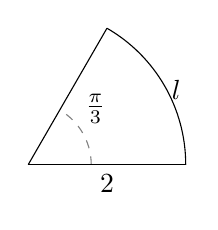
\begin{tikzpicture}
		\draw (2,0) arc (0:60:2);
		\draw[dashed,gray] (0.8,0) arc (0:60:0.8);
		\draw (0,0) -- (2,0);
		\draw (0,0) -- (1,1.732);
		
		\node[right] at (1.7,0.95) {$l$};
		\node[below] at (1,0) {$2$};
		\node[above right] at (0.6,0.4) {$\frac{\pi}{3}$};
	\end{tikzpicture}
	\end{center}
\item Calculate the arc lengths $l_1$, $l_2$ and area $A$ between the red curves in the diagram below:
	\begin{center}
	\begin{tikzpicture}
		\draw[red] (4,0) arc (0:240:4);
		\draw[dashed] (0,0) -- (4,0);
		\draw[dashed] (0,0) -- (-2,-3.46);
		
		\draw[red] (1,0) arc (0:240:1);
		\draw[red] (1,0) -- (4,0);
		\draw[red] (-0.5,-0.865) -- (-2,-3.46);
		
		\draw[dashed,gray] (1,0) arc (0:-120:1);
		\node[below right] at (0.5, -0.8) {$2.4$};
				
		\node[above left] at (-1, 4) {$l_1$};
		\node[above left] at (-0.4,0.9) {$l_2$};
		\node at (1,2) {$A$};
		
		\draw[<->] (1, 0.2) -- (4,0.2);
		\node[above] at (2.5,0.2) {$5$};
		\draw[<->] (0,0.2) -- (1, 0.2);
		\node[above] at (0.5, 0.2) {$1$};

	\end{tikzpicture}
	\end{center}
\item Find the angles $A$ and $B$ in the triangles below:
	\begin{center}
	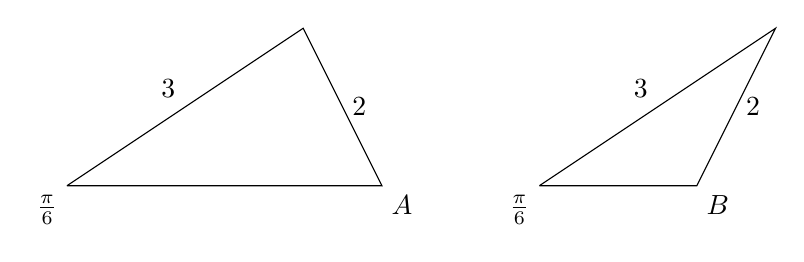
\begin{tikzpicture}
		\draw (0,0) -- (3,2) -- (4,0) -- (0,0);
		\node[above left] at (1.5,1) {$3$};
		\node[right] at (3.5,1) {$2$};
		\node[below left] at (0,0) {$\frac{\pi}{6}$};
		\node[below right] at (4,0) {$A$};
		
		\draw (6,0) -- (9,2) -- (8,0) -- (6,0);
		\node[above left] at (7.5,1) {$3$};
		\node[right] at (8.5,1) {$2$};
		\node[below left] at (6,0) {$\frac{\pi}{6}$};
		\node[below right] at (8,0) {$B$};
	\end{tikzpicture}
	\end{center}
\item Find the missing length in the triangle below, and the area:
	\begin{center}
	\begin{tikzpicture}
		\draw (0,0) -- (4,-3) -- (6,4) -- (0,0);
		\node[left] at (0,0) {$\frac{\pi}{3}$};
		\node[below left] at (2,-1.5) {$4$};
		\node[above left] at (3,2) {$6$};
	\end{tikzpicture}
	\end{center}
\item Solve $\cos^2(t)+\cos(t)=\sin^2(t)$ for $0\leq t<2\pi$.
\item Solve $\cosec(x)+a\sin(x)=b$ in terms of $a$ and $b$, for $0^\circ\leq x<360^\circ$.
\end{enumerate}









\clearpage

\textbf{Theory---Sums of Sinusoids of Equal Frequency:}

\vspace{5mm}

The compound angle formulae split a single sine or cosine into a combination of sines and cosines:
\[\sin(\alpha+\beta) = \sin(\alpha)\cos(\beta)+\cos(\alpha)\sin(\beta),\]
\[\cos(\alpha+\beta) = \cos(\alpha)\cos(\beta)-\sin(\alpha)\sin(\beta).\]
We can use this in reverse to combine sines and cosines \textbf{of the same frequency} into a single sine or cosine.

\vspace{5mm}

Write $3\cos(7\theta)-4\sin(7\theta)$ in the form $R\cos(7\theta+\alpha)$ for some $R$ and $\alpha$.

\vfill

Hence solve $3\cos(7\theta)-4\sin(7\theta)=\frac{1}{\sqrt{2}}$ for $0\leq \theta<\pi$.

\vfill



\clearpage








Here we show the graphs of the functions from the last page:

\begin{center}
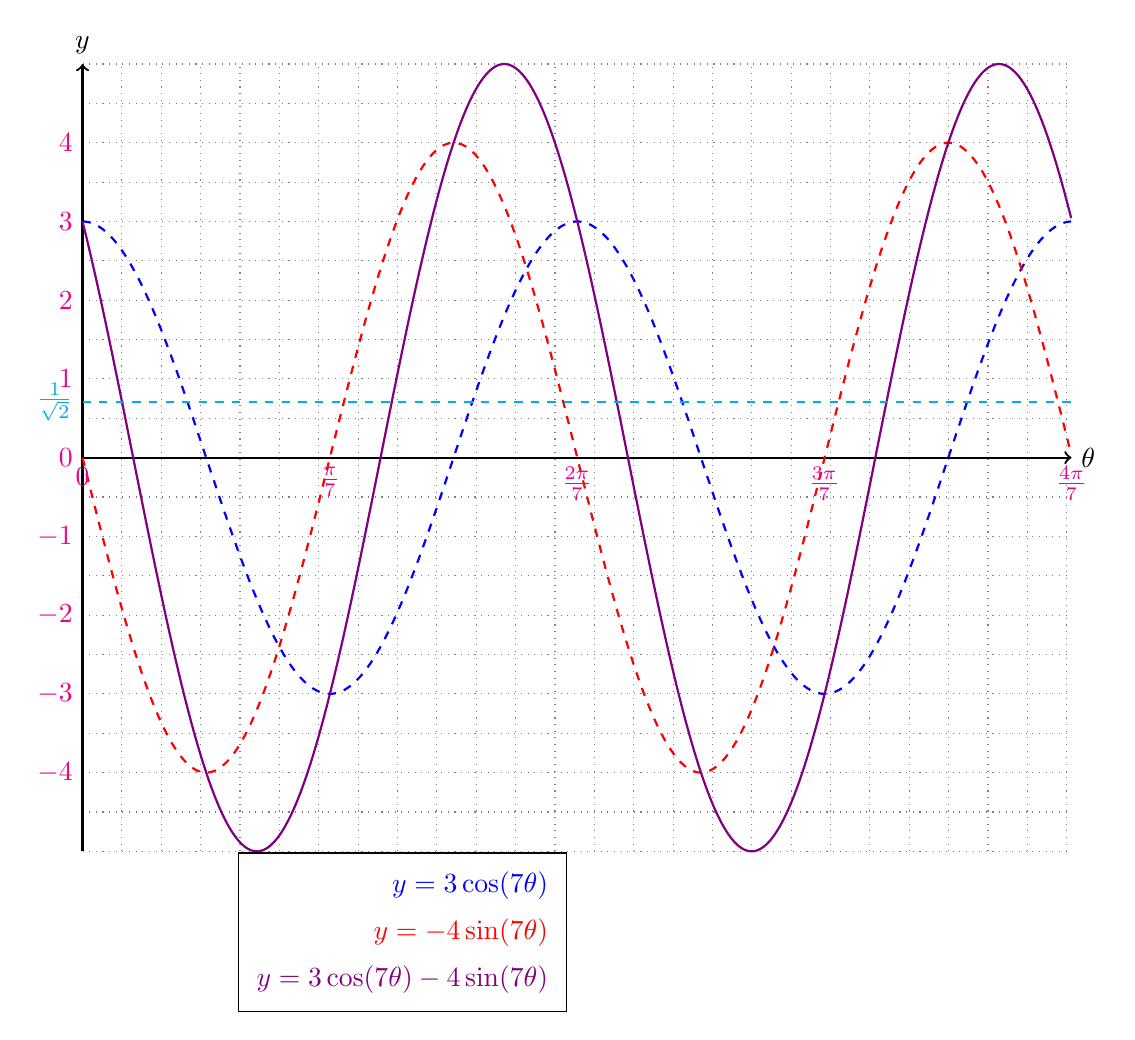
\begin{tikzpicture}
\draw[white] (0,0) -- (13,0);
\draw[step=0.5,gray,thin,dotted] (0,-5) grid (12.56,5);
\draw[thick, ->] (0,-5) -- (0,5);
\node[above] at (0,5) {$y$};
\draw[thick,->] (0,0) -- (12.56,0);
\node[right] at (12.56,0) {$\theta$};

\draw[blue,thick, dashed, domain=0:12.56, samples=300] plot (\x,{3*cos((\x) r)});
\draw[red,thick, dashed, domain=0:12.56, samples=300] plot (\x,{-4*sin((\x) r)});
\draw[violet,thick, domain=0:12.56, samples=300] plot (\x,{3*cos((\x) r) - 4*sin((\x) r)});

\node[magenta,below] at (0,0) {0};
\node[magenta,below] at (3.14,0) {$\frac{\pi}{7}$};
\node[magenta,below] at (6.28,0) {$\frac{2\pi}{7}$};
\node[magenta,below] at (9.42,0) {$\frac{3\pi}{7}$};
\node[magenta,below] at (12.56,0) {$\frac{4\pi}{7}$};


\foreach \i in {-4,-3,-2,-1,0,1,2,3,4}{
	\node[left,magenta] at (0,\i) {$\i$};
	}

	
\draw[cyan,dashed] (0,0.707) -- (12.56,0.707);
\node[cyan,left] at (0,0.707) {$\frac{1}{\sqrt{2}}$};
	
\matrix [draw,below left] at (current bounding box.south) {
	\node [blue] {$y=3\cos(7\theta)$}; \\
	\node [red] {$y=-4\sin(7\theta)$}; \\
	\node[violet] {$y=3\cos(7\theta)-4\sin(7\theta)$};\\
};
\end{tikzpicture}
\end{center}






\clearpage






\textbf{Practice:}

\vspace{5mm}


\begin{enumerate}
\item Express $\sin(3t)-\sqrt{3}\cos(3t)$ in the form $R\sin(3t-\alpha)$.
\item Solve the equation $6\cos(4x)+8\sin(4x) = -0.5$ for $0\leq x<\frac{\pi}{2}$.
\item The voltage of mains electricity varies with time by the function $230\sqrt{2}\sin(100\pi t)$. A drive coil on a so-called ``3-phase'' electric motor receives two alternating voltages, with a time offset between them:
\[A=230\sqrt{2}\sin(100\pi t),\qquad\qquad B=230\sqrt{2}\sin\left(100\pi t+\frac{2\pi}{3}\right).\]
The resulting voltage on the drive coil is $A-B$, the difference between these two voltages. Express the resulting voltage on the drive coil as a single sine function of time; \textit{i.e.}, write $A-B$ in the form $R\sin(100\pi t+\alpha)$. Hence suggest why for high-power applications 3-phase motors are used instead of single phase motors (with just one mains voltage applied).
\item Sound is a pressure wave in the air; for a single pure note at frequency $f$ and amplitude $A$, the pressure $P_1$ at a point in the air varies with time according to $P_1=A\sin(2\pi f t)$. When two sounds are played, with pressure waves $P_1$ and $P_2$, the overall effect on air pressure is $P_1+P_2$.

Suppose an additional sound is played, with $P_2=A\sin\left((2\pi+1) ft\right)$. The overall result of these two pressure waves is that the total air pressure is $P_{\mathrm{total}}=P_1+P_2$. Apply the compound angle formula for sine to $P_2$ and hence find $P_\mathrm{total}$. Describe the sound which results when both these sounds are played together, and hence suggest how noise-cancelling headphones work.
\end{enumerate}






\end{document}